\chapter{Περιγραφή υλοποίησης}


\section{Περιβάλλον ανάπτυξης}

Η επιλογή μικροελεγκτή (MCU) αντί μικροεπεξεργαστή (MPU) για την ανάληψη των
καθηκόντων της υλοποίησης θεωρείται δεδομένη.
Ως βασικά στοιχεία υπεροχής των μικροελεγκτών κρίνεται η χαμηλότερη κατανάλωση
ισχύος, η έλλειψη ανάγκης σύνδεσης και τροφοδοσίας εξωτερικής κύριας και
δευτερεύουσας μνήμης, και ο λιγότερος (φυσικός) χώρος που καταλαμβάνουν
\parencite[1--2]{atmel13:mpu-mcu}. Αυτά βέβαια παρέχονται εις βάρος χαμηλότερης
επεξεργαστικής ισχύος και λιγότερης μνήμης που, σε αντίθεση με τους
μικροεπεξεργαστές που υποστηρίζουν μεγέθη της τάξης των GiB, οι μικροελεγκτές
περιορίζονται σε μερικά MiB.

Βέβαια, παρότι ένας μικροελεγκτής είναι πιο συμπαγής, απαιτούνται, τελικά,
ορισμένα επιπρόσθετα στοιχεία όπως, για παράδειγμα, για τη ρύθμιση και
σταθεροποίηση της τάσης που αυτός λαμβάνει. Επιπλέον, τίθενται ζητήματα που
αφορούν τον προγραμματισμού του καθώς και τη (φυσική) διασύνδεση με τα
οποιαδήποτε εξαρτήματα και εξωτερικά ολοκληρωμένα που πρόκειται να
χρησιμοποιηθούν.


\subsection{Πλατφόρμα Arduino}
\label{subsec:arduino}

Οι πλακέτες Arduino επιλύουν τα παραπάνω ζητήματα και παρέχουν μία έτοιμη
λειτουργική μονάδα που επιτρέπει την άμεση ενασχόληση με τη δημιουργία του
πρότυπου λογισμικού και εκείνων των συνδέσεων με ηλεκτρονικά στοιχεία που
απαιτούνται στο πλαίσιο αυτού.

Για την ύπαρξη αρκετής ευελιξίας κατά το σχεδιασμό της υλοποίησης (και λόγω
έλλειψης πρότερης εμπειρίας και, επομένως, κρίσης), επιλέγεται η (πλέον
πρόσφατη, την περίοδο εκπόνησης) πλακέτα Arduino Uno revision 3, της οποίας ο
κεντρικός μικροελεγκτής είναι ένας AVR ATmega328P της Atmel. Ο συγκεκριμένος
μικροελεγκτής διαθέτει συνολική μνήμη προγράμματος 32KiB, 2KiB κύρια μνήμη,
συχνότητα ρολογιού που φτάνει τα 20MHz (που, ωστόσο, λόγω της πλακέτας,
περιορίζεται στα 16MHz) και πληθώρα δυνατοτήτων
\parencites[1]{atmel13}{arduino:uno}. Επιπροσθέτως, η πλακέτα παρέχει διασύνδεση
USB για την επικοινωνία του μικροελεγκτή με τον υπολογιστή, τόσο για τον
προγραμματισμό του όσο και για την ανταλλαγή δεδομένων με κάποια άλλη εφαρμογή,
για παράδειγμα τερματικό. Στο σχήμα \ref{fig:arduino:uno-front} παρουσιάζεται η
πλακέτα Arduino και τα βασικά της μέρη.

\begin{figure}
    \caption{Πλακέτα Arduino Uno.\label{fig:arduino:uno-front}}
    \begin{center}
    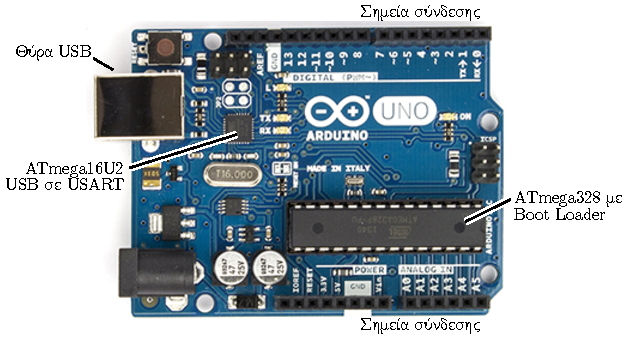
\includegraphics{arduino_uno}
    \end{center}
    Βασισμένο. \fullcite{arduino:uno:front}
\end{figure}

Ο μικροελεγκτής της πλακέτας \te{Arduino Uno revision 3} διατίθεται με
προεγκατεστημένο
λογισμικό \te{Boot loader} επιτρέποντας, με αυτόν τον τρόπο, τον προγραμματισμό
της μνήμης προγράμματος χωρίς τη χρήση ειδικού υλικού, αλλά με την απευθείας
σύνδεση της πλακέτα μέσω καλωδίου USB \parencite{arduino:environ}. Περισσότερα
σχετικά με το λογισμικό \te{Boot loader} αναφέρονται στην ενότητα
\nameref{subsec:avr:progmem} σ.~\pageref{subsec:avr:progmem}.
Ωστόσο, σημειώνεται ότι η
επικοινωνία μέσω USB επιτυγχάνεται με ένα δεύτερο μικροελεγκτή της πλακέτας --
ενός ATmega16U2 -- του οποίου μοναδικός σκοπός είναι η διασύνδεση του
πρωτοκόλλου USB (το οποίο υποστηρίζει εγγενώς) με το κύκλωμα USART που διαθέτει,
τόσο ο ίδιος, αλλά, κυρίως, ο ATmega328P -- ο κεντρικός μικροελεγκτής της
πλακέτας \parencites{arduino:uno}[148,185]{atmel12}[172]{atmel13}. Σαφώς, αυτή η
διασύνδεση χρησιμοποιείται για κάθε επικοινωνία μεταξύ υπολογιστή και πλακέτας
μέσω καλωδίου USB, ανεξαρτήτως εάν τα δεδομένα προορίζονται για το λογισμικό
\te{Boot loader} ή το ίδιο το πρόγραμμα.

Για την περαιτέρω διευκόλυνση της ανάπτυξης του λογισμικού του μικροελεγκτή της
πλακέτας,
παρέχεται ορισμένο επιπρόσθετο λογισμικό \te{Arduino} το οποίο λαμβάνει δύο
μορφές. Μία εξ αυτών είναι το περιβάλλον ανάπτυξης \te{Arduino IDE} του οποίου
οι βασικές λειτουργίες είναι η μεταγλώττιση του πηγαίου κώδικα και η μεταφορά
του προγράμματος στο μικροελεγκτή \parencite{arduino:environ} μέσω μίας
περισσότερο ελκυστικής γραφικής διεπαφής. Μία δεύτερη μορφή
λογισμικού είναι οι βιβλιοθήκες \te{Arduino} οι οποίες παρέχουν εύχρηστες
προγραμματιστικές διεπαφές (API) που εσωτερικά κάνουν χρήση των υποκείμενων
κυκλωμάτων του μικροελεγκτή της εκάστοτε πλακέτας (είτε απευθείας, είτε μέσω
τρίτου λογισμικού) αποκρύπτοντας, με αυτόν τον τρόπο, τις λεπτομέρειες της
υλοποίησης \parencite{arduino:lib}.


\subsubsection{Εργαλεία προγραμματισμού}
\label{subsubsec:avr:toolchain}

Παρότι το IDE και οι βιβλιοθήκες Arduino μπορούν να επιταχύνουν σημαντικά τη
διαδικασία ανάπτυξης της υλοποίησης, προτιμάται, αντί αυτών, η απευθείας χρήση
καθιερωμένων εργαλείων για τον προγραμματισμό μικροελεγκτών AVR, καθώς έτσι
επιδιώκεται να επιτευχθεί σε μεγαλύτερο βάθος κατανόηση της συνολικής
διαδικασίας που, ιδανικά, θα επιτρέψει τη μελλοντική ενασχόληση με παρόμοια
συστήματα ανεξαρτήτως της πορείας των προϊόντων \te{Arduino}. Στο πλαίσιο της
υλοποίησης, χρησιμοποιείται μόνο το υλικό, δηλαδή η πλακέτα \te{Arduino} για την
κάλυψη των βασικών ηλεκτρικών αναγκών, και το λογισμικό \te{Boot loader} για τον
προγραμματισμό του μικροελεγκτή καθώς και το λογισμικό του ATmega16U2 το οποίο
διασυνδέει τον κεντρικό μικροελεγκτή με τη θύρα USB.

Το IDE αντικαθίσταται από έναν οποιοδήποτε επεξεργαστή κειμένου και ο πηγαίος
κώδικας διασπάται σε διαφορετικά αρχεία για την καλύτερη οργάνωσή του.
Με τον τρόπο αυτό, καθώς η υλοποίηση επεκτείνεται και ο κώδικάς της διογκώνεται,
ο λογικός διαχωρισμός των λειτουργιών της επιτρέπει το γρηγορότερο εντοπισμό
κάποιας συγκεκριμένης υπομονάδας. Επιπλέον, καθώς η μεταγλώττιση μεγάλου όγκου
πηγαίου κώδικα μπορεί να αποβεί χρονοβόρα, η ύπαρξη αυτόνομων αρχείων
αντικείμενου προγράμματος δημιουργημένων από προηγούμενο κύκλο μεταγλώττισης,
επιτρέπει την επαναχρησιμοποίησή τους για την παραγωγή ενός (νέου) συνολικού
δυαδικού αρχείου, απαιτώντας μεταγλώττιση μόνο των αρχείων εκείνων που έχουν
τροποποιηθεί.

Η μεταγλώττιση των επιμέρους αρχείων πηγαίου κώδικα σε αντικείμενα προγράμματα
και η, εν συνεχεία, σύνδεση (ή συνένωσή) τους σε ένα τελικό δυαδικό αρχείο
αναλαμβάνεται από την AVR GNU συλλογή μεταγλωττιστών avr-gcc και λοιπών
εργαλείων της avr-binutils (όπως ο συνδέτης ld ο οποίος χρησιμοποιείται
εσωτερικά από την avr-gcc). Η σύνταξη του κώδικα γίνεται σε γλώσσα C με τη
βοήθεια της βιβλιοθήκης AVR Libc.

Το παραγόμενο δυαδικό αρχείο της σύνδεσης είναι μορφής ELF (\te{Executable and
Linking Format}) η οποία, παρότι παρέχει ανεξαρτησία από επεξεργαστή και
αρχιτεκτονική υπολογιστή, είναι, ωστόσο ακατάλληλη για την απευθείας μεταφορά
στο μικροελεγκτή AVR \parencites[47]{cruz97}[346]{avrlibc}. Απαιτείται, πρώτα, η
εξαγωγή των τμημάτων (\te{segment}) του κώδικα και των δεδομένων (\@.\te{text}
και \@.\te{data}, αντίστοιχα) από το αρχείο ELF σε ένα αρχείο δεκαεξαδικής
μορφής (αρχείο HEX) · εργασία η οποία αναλαμβάνεται από το εργαλείο avr-objcopy
\parencite[13,346]{avrlibc}.

\begin{figure}
    \caption{Η αλυσίδα εργαλείων AVR GCC για τον προγραμματισμό του
    μικροελεγκτή.\label{fig:avr:toolchain}}
    \begin{center}
    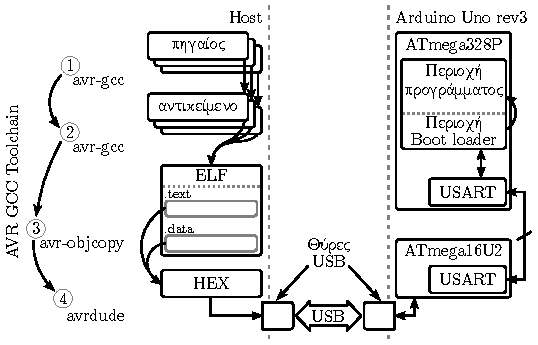
\includegraphics{avr_toolchain}
    \end{center}
\end{figure}

Τέλος, το δεκαεξαδικό αρχείο περνάει στο μικροελεγκτή μέσω του εργαλείου
avrdude, το
οποίο υποστηρίζει προγραμματισμό μικροελεγκτών AVR μέσω διαφόρων προγραμματιστών
(συμπεριλαμβανομένου ειδικών εξαρτημάτων όπως οι STK500 και AVRISP mkII της
Atmel) και, σαφώς, μέσω \te{Boot loader} \parencites[15]{avrlibc}{avrdude}.

Σημειώνεται ότι, γενικά, η χρήση \te{Boot loader} περιορίζεται στην εγγραφή και
ανάγνωση της μνήμης \te{Flash} και EEPROM χωρίς να παρέχεται η δυνατότητα
εγγραφής των λεγόμενων \te{fuse bit}, τα οποία πρόκειται για μη πτητικές θέσεις
μνήμης που ρυθμίζουν, με διάφορους τρόπους, τη συμπεριφορά του μικροελεγκτή
όπως, για παράδειγμα, το μέγεθος της περιοχής \te{Boot loader} (σχετικά με
αυτήν, βλ. \nameref{subsec:avr:progmem} σ.~\pageref{subsec:avr:progmem})· κάτι
τέτοιο είναι δυνατό μόνο μέσω σειριακών ή παράλληλων συνδέσεων προγραμματισμού
\parencite[273]{atmel13}.  Επιπλέον, στην περίπτωση του \te{Boot loader} του
Arduino Uno revision 3, παρέχεται εγγραφή αποκλειστικά και μόνο για τη μνήμη
προγράμματος (μνήμη \te{Flash}), κυρίως για τη μείωση του μεγέθους του.


\subsubsection{Εντολές προγραμματισμού}

Στο σχήμα \ref{fig:avr:toolchain} παρουσιάζεται η αλυσίδα (\te{toolchain}) των
χρησιμοποιούμενων εργαλείων για τη μετάβαση από κάθε στάδιο στο επόμενο με
τελικό στόχο τον προγραμματισμό του μικροελεγκτή. Στη βασική τους μορφή, οι
εντολές συνοψίζονται παρακάτω.

\begin{enumerate}

    \item Μετατροπή αρχείων πηγαίου σε αρχεία αντικείμενου προγράμματος για κάθε
    αρχείο \verb~file.c~. Τυπικά, η εντολή εκτελείται μόνο για εκείνα τα αρχεία
    πηγαίου κώδικα που έχουν τροποποιηθεί.

\begin{lstlisting}
avr-gcc -mmcu=atmega328 -Wl,-Map,mcu.map -Os -c file.c
\end{lstlisting}

    \begin{description}
        \item[-mmcu] Καθορίζει τον τύπο του μικροελεγκτή ώστε να αναγνωρίζεται
        το κατάλληλο σύνολο εντολών (\te{instruction set}) που πρόκειται να
        χρησιμοποιηθεί κατά τη συμβολομετάφραση \parencite{gcc:options}.

        \item[-Os] Ενεργοποιεί τις βελτιστοποιήσεις του κώδικα από το
        μεταγλωττιστή προκειμένου να εξοικονομηθεί χώρος προγράμματος, ακόμα και
        εις βάρος της ταχύτητας εκτέλεσής του (Optimize for size)
        \parencites[338]{avrlibc}{gcc:options}.

        Εκτός του άμεσου πλεονεκτήματος της παραγωγής μικρότερου προγράμματος, η
        συγκεκριμένη ρύθμιση απαιτείται από τη βιβλιοθήκη AVR Libc προκειμένου
        να διατίθενται ορισμένες λειτουργίες προσωρινής «παύσης» της εκτέλεσης
        του προγράμματος (βρόχοι \te{busy-wait}) \parencite[328]{avrlibc}.

        \item[-c] Η συγκεκριμένη επιλογή προκαλεί την παραγωγή αρχείου
        αντικείμενου προγράμματος όπως αυτό εξάγεται από το συμβολομεταφραστή,
        αποτρέποντας τη σύνδεσή του σε τελικό πρόγραμμα
        \parencites[338]{avrlibc}{gcc:options}.
    \end{description}


    \item Σύνδεση των αρχείων αντικείμενου προγράμματος σε αρχείο ELF.
\begin{lstlisting}
avr-gcc -mmcu=atmega328 *.o -o mcu.elf
\end{lstlisting}

    \begin{description}
        \item[-mmcu] Ομοίως με την προηγούμενη εντολή.

        \item[-o] Καθορίζει το όνομα του παραγόμενου αρχείου
        \parencite{gcc:options}.
    \end{description}


    \item Μετατροπή αρχείου ELF σε δεκαεξαδική μορφή Intel HEX.
\begin{lstlisting}
avr-objcopy -j .text -j .data -O ihex mcu.elf mcu.hex
\end{lstlisting}

    \begin{description}
        \item[-j] Καθορίζει ποια τμήματα του αρχείου ELF θα χρησιμοποιηθούν για
        τη δημιουργία του αρχείου εξόδου. Στην προκειμένη, εξάγεται ο κώδικας
        και τα δεδομένα \parencite[346]{avrlibc}.

        \item[-O] Καθορίζει τον τύπο του παραγόμενου αρχείου
        \parencite[346]{avrlibc}. Στην περίπτωση του μικροελεγκτή AVR, πρόκειται
        για ένα αρχείο κειμένου ASCII του οποίου τα δεκαεξαδικά ψηφία
        κωδικοποιούν, ένα προς ένα, τα Byte του αρχικού δυαδικού αρχείου το
        οποίο αποτελεί το πρόγραμμα που εγγράφεται στη μνήμη Flash
        \parencites[4]{intel88}[10]{atmel12programmer}.
    \end{description}


    \item Αποστολή αρχείου HEX στο λογισμικό \te{Boot loader} του μικροελεγκτή
    για τη μετέπειτα εγγραφή του στην περιοχή προγράμματος (βλ.
    \nameref{subsec:avr:progmem} σ.~\pageref{subsec:avr:progmem}).
\begin{lstlisting}
avrdude -p atmega328p -c arduino -P /dev/ttyACM0 -b 115200 -U flash:w:mcu.hex:i
\end{lstlisting}
    \begin{description}
        \item[-p] Το μοντέλο του μικροελεγκτή, το οποίο στην περίπτωση της
        υλοποίησης είναι ο ATmega328P.

        \item[-c] Ο χρησιμοποιούμενος προγραμματιστής, ώστε να αναγνωρίζεται η
        συνδεσμολογία με το μικροελεγκτή και να εφαρμόζονται τα κατάλληλα
        σήματα ελέγχου.

        \item[-P] Η θύρα του υπολογιστή στην οποία είναι συνδεδεμένος ο
        προγραμματιστής. Στην περίπτωση της υλοποίησης όπου χρησιμοποιείται
        \te{Boot loader}, η θύρα σύνδεσης είναι USB η οποία, στο σύστημα του
        υπολογιστή, εμφανίζεται ως \slash{}dev\slash{}ttyACM0.

        \item[-b] Ο ρυθμός baud μετάδοσης δεδομένων μέσω της σειριακής. Σύμφωνα
        με τις προδιαγραφές του Arduino Uno, ο χρησιμοποιούμενος \te{Boot
        loader} λειτουργεί στα 115200Bd \parencite{arduino:environ}.

        \item[-U] Ο τύπος της εργασίας που πρόκειται να εκτελεστεί. Το πρόγραμμα
        avrdude μπορεί να χρησιμοποιηθεί τόσο για την εγγραφή όσο και για την
        ανάγνωση των διαθέσιμων μνημών του εκάστοτε μικροελεγκτή (για
        παράδειγμα, \te{Flash}, EEPROM, \te{fuse}), εφόσον αυτό υποστηρίζεται%
        \slash{}επιτρέπεται από τον μικροελεγκτή \parencite{avrdude}. Στο
        πλαίσιο της υλοποίησης, ενδιαφέρει μόνο η εγγραφή (\verb~w~) της μνήμης
        \te{Flash} με τα δεδομένα του αρχείου HEX (μορφής \verb~i~ntel).
    \end{description}

\end{enumerate}


\subsection{Λοιπό λογισμικό ανάπτυξης}

Πέραν των εργαλείων της συλλογής AVR GCC που περιγράφονται στην ενότητα
\nameref{subsubsec:avr:toolchain} (σ.~\pageref{subsubsec:avr:toolchain}),
χρησιμοποιούνται και ορισμένα άλλα. Όλα πρόκειται για Ελεύθερο λογισμικό αδείας
συμβατής είτε με την άδεια GNU GPL είτε την LGPL, με τα περισσότερα να
υποστηρίζουν πολλαπλά λειτουργικά συστήματα πέραν των βασισμένων σε \te{UNIX}.

\begin{description}

\item[Make]
Εργαλείο αυτοματισμού της ενημέρωσης παρακολουθούμενων αρχείων, αναγνωρίζει,
βάσει κανόνων που του δηλώνει ο χρήστης, ποια αρχεία έχουν τροποποιηθεί και
ενεργοποιεί τις αντίστοιχες εντολές για την ενημέρωσή αυτών καθώς και πιθανών
άλλων αρχείων εξαρτώμενων από αυτών που μόλις ενημερώθηκαν
\parencite{make:intro}.

Στο πλαίσιο της
υλοποίησης, χρησιμοποιείται για την εκ νέου μεταγλώττιση μόνο εκείνων των
αρχείων πηγαίου κώδικα που έχουν τροποποιηθεί, παράγοντας τα αντίστοιχα αρχεία
αντικείμενου προγράμματος και την, εν συνεχεία, σύνδεσή τους για την παραγωγής
του αρχείου HEX. Επίσης, περιλαμβάνει τη μεταφορά του αρχείου στο μικροελεγκτή
καθώς και τη σύνταξη της τεκμηρίωσης (βλ. επόμενο εργαλείο).


\item[\LaTeX]
Σύστημα προετοιμασίας εγγράφων υψηλής τυπογραφικής αξίας, ορίζει ειδική σήμανση
κειμένου που χρησιμοποιείται για το χαρακτηρισμό του κειμένου και μέσω ορισμένων
εργαλείων, παράγεται το τελικό έγγραφο \parencite{latex}. Η παρουσίαση\slash{}%
εμφάνιση του εγγράφου (όπως περιθώρια, διατάξεις) καθορίζεται από,
τροποποιήσιμους έως ένα βαθμό, προκαθορισμένους εσωτερικούς κανόνες του
συστήματος \LaTeX{}  που έχουν δημιουργηθεί ώστε να ευνοείται η αναγνωσιμότητα
του τελικού προϊόντος.

Το σύστημα \LaTeX και τα σχετικά εργαλεία χρησιμοποιούνται για τη σύνταξη της
τεκμηρίωσης (του παρόντος εγγράφου). Μεταξύ άλλων, διευκολύνεται η εργασία με
αναφορές, τόσο μεταξύ μερών του εγγράφου όσο και των βιβλιογραφικών αναφορών και
η διατύπωση μαθηματικών παραστάσεων. Επίσης, καθώς ο επεξεργαστής κειμένου είναι
υπεύθυνος για την εμφάνιση μόνο κειμένου, η απόκριση του είναι ταχύτερη και ο
χειρισμός του πιο αποτελεσματικός.

Τέλος, επειδή τα αρχεία είναι κειμένου και όχι δυαδικά, οι αλλαγές που
πραγματοποιούνται σε αυτά είναι δυνατό να παρακολουθούνται από το σύστημα
παρακολούθησης αλλαγών σε επίπεδο γραμμής (βλ. επόμενο εργαλείο).

\item[Git]
Σύστημα παρακολούθησης αλλαγών το οποίο χαρακτηρίζεται για την ταχύτητα
τη μικρή επιβάρυνση σε πόρους συστήματος και την ευελιξία του \parencite{git}.
Επιτρέπει, μεταξύ άλλων, την καταγραφή των αλλαγών που πραγματοποιούνται σε
αρχεία της υλοποίησης (κατά κύριο λόγο, του πηγαίου κώδικα υλοποίησης και
τεκμηρίωσης) και παρέχει τη δυνατότητα πραγματοποίησης εύκολα αναστρέψιμων
πειραματικών αλλαγών.
Επιπλέον, παρέχει μία εύληπτη παρουσίαση πορείας των εργασιών που έχουν
πραγματοποιηθεί.

\item[Doxygen]
Λογισμικό παραγωγής τεκμηρίωσης πηγαίου κώδικα μέσω ειδικών σημάνσεων που
εισάγονται στα σχόλιά του, κυρίως απευθυνόμενο σε κώδικα γλώσσας C και C++
\parencite{doxygen}. Το σύνολο του πηγαίου κώδικα της υλοποίησης (για
παράδειγμα, συναρτήσεις, δομές, μεταβλητές) τεκμηριώνεται σύμφωνα με τις οδηγίες
του \te{Doxygen} ώστε να είναι δυνατή η δημιουργία ενός, ηλεκτρονικής μορφής,
προγραμματιστικού εγχειριδίου των επιμέρους μονάδων (\te{module}) για την
υποστήριξη της κατανόησης της λειτουργίας του καθενός και τη διευκόλυνση της
ενσωμάτωσης τους σε πιθανές άλλες υλοποιήσεις.

\item[Qucs]
Λογισμικό με γραφικό περιβάλλον (GUI) για τη δημιουργία και προσομοίωση
κυκλωμάτων, με δυνατότητα απεικόνισης των αποτελεσμάτων των προσομοιώσεων σε
διάφορες μορφές, όπως γραφήματα \parencite{qucs}.
Χρησιμοποιείται για το σχεδιασμό του προτύπου της διασύνδεσης του μικροελεγκτή
με όλα τα ολοκληρωμένα κυκλώματα και τα συμπληρωματικά στοιχεία της υλοποίησης.
Επιλέγεται, κυρίως, λόγω της ευκολίας με την οποία δημιουργούνται προσαρμοσμένα
κυκλώματα και επειδή υποστηρίζει την εξαγωγή των κυκλωμάτων σε διανυσματική
μορφή που εύκολα ενσωματώνεται στο έγγραφο της τεκμηρίωσης, δίχως απώλειες στην
ποιότητά τους.

\item[Inkscape]
Λογισμικό σχεδίασης διανυσματικών γραφικών \parencite{inkscape}. Χρησιμοποιείται
για τη δημιουργία όλων των επεξηγηματικών σχημάτων της τεκμηρίωσης για το λόγο
ότι επιτρέπει γρήγορη σχεδίαση γραφικών υψηλής ευκρίνειας με δυνατότητα εύκολης
ενσωμάτωσης στην τεκμηρίωση.

\item[Blender3D]
Ολοκληρωμένη σουίτα δημιουργίας τρισδιάστατων γραφικών \parencite{blender3d}.
Στο πλαίσιο της υλοποίησης, χρησιμοποιείται στο κομμάτι της κατασκευής της
συσκευής, τόσο για το σχεδιασμό και εξέταση προτύπων όσο και για την εξαγωγή
απεικονίσεων του εφαρμοσμένου προτύπου που περιλαμβάνονται, κυρίως, στο κεφάλαιο
\nameref{ch:construction} (σ.~\pageref{ch:construction}).

\item[Gimp]
Λογισμικό επεξεργασίας εικόνας \parencite{gimp}. Χρησιμοποιείται για τη βελτίωση
των χαρακτηριστικών ορισμένων εικόνων (για παράδειγμα, αντίθεση, κορεσμός), ώστε
να παρέχεται καλύτερο οπτικό αποτέλεσμα.
\end{description}


\section{Μικροελεγκτής}

Σύμφωνα με τον \textcite[1]{myklebust97}, οι μικροελεγκτές AVR διαθέτουν
μειωμένο σύνολο εντολών, δηλαδή είναι υπολογιστές RISC (\te{Reduced Instruction
Set Computer}). Το χαρακτηριστικό αυτό απλοποιεί τα απαιτούμενα κυκλώματα
ελέγχου και τους παρέχουν μικρότερους κύκλους για την εκτέλεση κάθε εντολής
\parencite[1]{sequin82}. Επιπροσθέτως, οι μικροελεγκτές AVR βασίζονται σε
τροποποιημένη αρχιτεκτονική Harvard σύμφωνα με την οποία, και σε αντίθεση με την
κατά Von Neumann αρχιτεκτονική, το πρόγραμμα και τα δεδομένα τοποθετούνται σε
ανεξάρτητα φυσικά μέσα που χαρακτηρίζονται, μεταξύ άλλων, από ανεξάρτητους
διαύλους πρόσβασης \parencite[1]{myklebust97}.

Άμεσα πλεονεκτήματα αυτού του σχεδιασμού είναι ότι καθίσταται δυνατή η
ταυτόχρονη πρόσβαση στις μνήμες προγράμματος και δεδομένων στον ίδιο κύκλο
\parencite[8]{atmel13}. Επιπλέον, επιτρέπεται η χρήση διαφορετικών τεχνολογιών
για κάθε μνήμη. Για παράδειγμα, στην περίπτωση του χρησιμοποιούμενου
μικροελεγκτή, ATmega328P, τα δεδομένα οργανώνονται σε μνήμη πλάτους των 8bit
τεχνολογίας SRAM (\te{Static RAM}) με 2KiB συνολική χωρητικότητα, ενώ οι
εντολές, σε μνήμη Flash των 32KiB με θέσεις των 16bit
\parencite[8--9,16,18]{atmel13}.


\subsection{Μνήμη προγράμματος}
\label{subsec:avr:progmem}

Η μνήμη Flash του μικροελεγκτή χωρίζεται σε δύο περιοχές λογισμικού, την περιοχή
του προγράμματος (\te{Application section}) και την περιοχή του λογισμικού
\te{Boot loader} (\te{Boot Loader Section} -- BLS) \parencite[269]{atmel13}.
Η περιοχή προγράμματος φέρει τον κώδικα που εκτελεί ο μικροελεγκτής κατά την
τυπική του λειτουργία· τον κώδικα της υλοποίησης. Στην περιοχή BLS εναποτίθεται
λογισμικό το οποίο μπορεί να εγγράψει και να διαβάσει τη μνήμη Flash με δεδομένα
που μεταφέρονται μέσω κάποιας διαθέσιμης διεπαφής του μικροελεγκτή (για
παράδειγμα, USART ή SPI), που, τυπικά, χρησιμοποιείται για την εναπόθεση του
νέου κώδικα του προγράμματος \parencite[269,273]{atmel13}.

Η εκτέλεση του \te{Boot loader} πραγματοποιείται είτε με την μεταπήδηση (εντολές
JMP ή CALL) στην περιοχή BLS από την περιοχή προγράμματος, είτε μέσω μίας
ρύθμισης του μικροελεγκτή που προκαλεί τη χρήση ως ρουτίνα εξυπηρέτησης της
διακοπής επανεκκίνησης (\te{Reset}), την πρώτη διεύθυνση της περιοχής BLS αντί
της πρώτης εντολής του προγράμματος, \parencite[273]{atmel13}. Από εκεί, το
λογισμικό \te{Boot loader} είναι υπεύθυνο να αποφασίσει εάν απαιτείται εγγραφή
νέου κώδικα στην περιοχή προγράμματος ή απευθείας μεταπήδηση πίσω σε αυτήν.

Το μέγεθος της περιοχής BLS είναι ρυθμιζόμενο και, στην περίπτωση του ATmega328,
δύναται να καταλαμβάνει τις τελευταίες 256, 512, 1024 ή 2048 λέξεις της μνήμης
Flash \parencite[282]{atmel13}. Στην περίπτωση του \te{Arduino Uno revision 3},
το λογισμικό \te{Boot loader} καταλαμβάνει 512KiB \parencite{arduino:uno}.


\subsection{Καθήκοντα μικροελεγκτή}

Κατά την εκκίνηση της συσκευής, δηλαδή κατά τη σύνδεσή της με την παροχή
τροφοδοσίας και, για λόγους που αναφέρονται στις ενότητες
\nameref{subsec:arduino} (σ.~\pageref{subsec:arduino}) και
\nameref{subsec:avr:progmem} (σ.~\pageref{subsec:avr:progmem}), αφιερώνονται
μερικά δευτερόλεπτα για την εκκίνηση πιθανού προγραμματισμού του μικροελεγκτή.
Στην τυπική λειτουργία της συσκευής, αυτό γίνεται αντιληπτό ως μία μικρή
καθυστέρηση κατόπιν της οποίας, εκτελείται η αρχικοποίηση των διαφόρων
υποσυστημάτων της
υλοποίησης
και, εν συνεχεία, ο μικροελεγκτής μεταπίπτει σε κατάσταση χαμηλής κατανάλωσης
ισχύος. Από αυτήν, ενεργοποιείται αυτόματα είτε για την εκκίνηση ενός νέου
κύκλου μετρήσεων (βλ. \nameref{sec:task} σ.~\pageref{sec:task}), είτε για την
εξυπηρέτηση κάποιου εισερχόμενου αιτήματος HTTP (βλ. \nameref{%
sec:network:impl-resources} σ.~\pageref{sec:network:impl-resources}). Στο σχήμα
\ref{fig:mcu:tasks} παρουσιάζεται ο κύκλος καθηκόντων του μικροελεγκτή.

\begin{figure}
    \caption{Καθήκοντα του μικροελεγκτή.\label{fig:mcu:tasks}}
    \begin{center}
    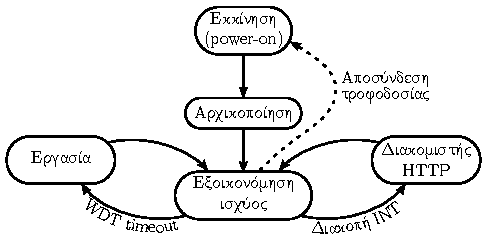
\includegraphics{mcu_tasks}
    \end{center}
\end{figure}

Αναλυτικότερα, κατά το στάδιο της αρχικοποίησης, τίθεται η συχνότητα του
ρολογιού του μικροελεκτή, η οποία, για τις ανάγκες της υλοποίησης, μειώνεται από
τα 16MHz στα 4MHz, και η κατεύθυνση των ακροδεκτών (δηλαδή ποιοι είναι εισόδου
και ποιοι εξόδου). Επίσης, ρυθμίζεται το κύκλωμα WDT (\te{Watch-Dog Timer}), το
οποίο είναι υπεύθυνο για την περιοδική αφύπνιση του μικροελεγκτή ώστε να
ελέγχεται η ανάγκη εκκίνησης νέου κύκλου μετρήσεων.

Επιπλέον, ανακτώνται οι μεταβλητές ρυθμίσεις της συσκευής είτε από τις
προκαθορισμένες (εργοστασιακές ρυθμίσεις), είτε από τις αποθηκευμένες τιμές της
εφεδρικής μνήμης, εφόσον αυτές είναι έγκυρες (βλ \nameref{subsec:backup-memory}
σ.~\pageref{subsec:backup-memory}).
Οι ρυθμίσεις αυτές περιλαμβάνουν τη δικτύωση της συσκευής (διεύθυνση IP, μάσκα
υποδικτύου, προεπιλεγμένη πύλη), το λειτουργικό εύρος του υποσυστήματος κίνησης
(βλ. \nameref{sec:motor:coordinates} σ.~\pageref{sec:motor:coordinates}), το
χρονικό διάστημα μεταξύ κύκλων εργασίας καθώς και το πλήθος μετρήσεων που
πραγματοποιείται σε κάθε κύκλο (βλ. \nameref{sec:task} σ.~\pageref{sec:task}).
Ο τρόπος ρύθμισης της συσκευής περιγράφεται στους Πόρους υλοποίησης (σ.~%
\pageref{sec:network:impl-resources}).

Στην πορεία, οι ρυθμίσεις προωθούνται στις κατάλληλες μονάδες και εκτελούνται
επιπρόσθετες προετοιμασίες, όπως η παλιννόστηση της κεφαλής, δηλαδή η επαναφορά
της στη θέση επιστροφής (συντεταγμένες [0, 0, Z\tsub{max}]) (βλ. σ.~%
\pageref{sec:motor:homing}) και η αρχικοποίηση του HTTP \te{Socket} (βλ. σ.~%
\pageref{ssubsec:network:port_mr}).


\subsection{Κατάσταση χαμηλής κατανάλωσης}

Ο μικροελεγκτής διαθέτει διάφορες καταστάσεις νάρκης (\te{sleep mode}
όπου η καθεμία απενεργοποιεί ορισμένα κυκλώματα για τη μείωση της κατανάλωσης.
Για παράδειγμα, η πιο απλή, είναι η κατάσταση αδράνειας (\te{idle}) κατά την
οποία απενεργοποιείται μόνο το ρολόι της CPU και της μνήμης Flash (δηλαδή, της
μνήμης προγράμματος). Στο πλαίσιο της υλοποίησης, γίνεται προσπάθεια για την
ύψιστη μείωση της κατανάλωσης κατά τα διαστήματα όπου ο μικροελεγκτής παραμένει
άεργος.

Για το σκοπό αυτό, εφαρμόζεται η κατάσταση \te{power-down} κατά την οποία
απενεργοποιούνται όλα τα ρολόγια του μικροελεγκτή (clk\tsub{CPU}, clk%
\tsub{FLASH}, clk\tsub{IO}, clk\tsub{ADC}, clk\tsub{ASY}) καθώς και οι
ταλαντωτές του συστήματος και των Χρονομετρητών\slash{}Απαριθμητών \parencite%
[38]{atmel13}. Σύμφωνα με την \textcite[38]{atmel13}, ο μικροελεγκτής είναι
δυνατό να επανέλθει σε κανονική λειτουργία μόνο μέσω των ακροδεκτών INT1:0 με
παρατεταμένο λογικό 0 (\te{low-level interrupt}) καθώς και μέσω των κυκλωμάτων
TWI (\te{Two-Wire Interface}) και WDT (\te{Watch-Dog Timer}).

Στο πλαίσιο της υλοποίησης χρησιμοποιείται ο πρώτος και ο τελευταίος τρόπος· το
κύκλωμα TWI αφυπνίζει το μικροελεγκτή όταν αυτός ρυθμίζεται με ρόλο \te{slave}
στο δίαυλο TWI και κάποιο εξωτερικό κύκλωμα προσπαθεί να επικοινωνήσει μαζί του
ενώ, στην υλοποίηση, χρησιμοποιείται μόνο ως \te{master} για την επικοινωνία με
το ρολόι πραγματικού χρόνου (RTC) (βλ. \nameref{sec:rtc} σ.~\pageref{sec:rtc}).

Για την ακρίβεια, ο ένας εκ των δύο ακροδεκτών INT1:0 συνδέεται με τον ακροδέκτη
\nbar{INT} του ολοκληρωμένου δικτύωσης, W5100, το οποίο τον θέτει και τον
διατηρεί σε λογικό 0 έως ότου διευθετηθούν όλες οι ενδείξεις διακοπών που του
έχουν ενεργοποιηθεί
(βλ. \nameref{subsec:network:interface} σ.~\pageref{subsec:network:interface}).
Για τις ανάγκες της υλοποίησης, αυτό σημαίνει ότι έχει καταφθάσει εισερχόμενο
αίτημα HTTP το οποίο διεκπεραιώνεται από το διακομιστή (βλ.
\nameref{sec:http-server} σ.~\pageref{sec:http-server}).

Ο χρονομετρητής WDT ρυθμίζεται ώστε να αφυπνίζει το μικροελεγκτή κάθε 8s (το
μέγιστο διάστημα που υποστηρίζεται από τον παρόντα μικροελεγκτή) και αποτελεί το
έναυσμα για την εκκίνηση νέου κύκλου εργασιών
(\nameref{ssubsec:task:initiate} σ.~\pageref{ssubsec:task:initiate}).


\section{Η υλοποίηση συνοπτικά}


\subsection{Κατασκευή}

Η κατασκευή της συσκευής γίνεται με χρήση ανοικτού (\te{open hardware})
συστήματος κατασκευής (\te{construction framework}), το \te{Open\-Builds}, για
την παροχή διαφόρων διευκολύνσεων (ράγες κίνησης, γραμμική κίνηση).

Η συσκευή είναι εμπνευσμένη από τη διάταξη κινητού γεφυρώματος (\te{moving
gantry}) εργαλειομηχανών CNC για την επίλυση των αναγκών της για γραμμική κίνηση
στο χώρο, με εξαίρεση ότι αφαιρείται η τράπεζα.
%Οι διαστάσεις της συσκευής είναι
Η κίνηση αφορά την κεφαλή, ένα εξάρτημα που φέρει αισθητήρες, και μετακινείται
σε επίπεδο πάνω από την επιφάνεια του παρακολουθούμενο υλικού και κατακόρυφα
προς αυτό για την πραγματοποίηση μετρήσεων. Η ύπαρξη της κινητής κεφαλής
επιτρέπει την αξιοποίηση ενός μικρού αριθμού αισθητήρων για την κάλυψη όλου του
παρακολουθούμενου υλικού. (Bλ. \nameref{ch:construction} σ.~%
\pageref{ch:construction}.)


\subsection{Κωδικοποίηση κίνησης}

Η μετατόπιση της κεφαλής πραγματοποιείται από κινητήρες. Η κίνησή τους
παρακολουθείται από κωδικοποιητή περιστροφικής κίνησης, ο οποίος παρέχει
ανατροφοδότηση στο μικροελεγκτή για τα, αναφερόμενα ως, βήματα που πραγματοποιεί
ο παρακολουθούμενος κινητήρας ώστε να αναγνωρίζει το μέγεθος της μετατόπισης.
Τέσσερα τέτοια βήματα (ή παλμοί) αποτελούν μία πλήρη περιστροφή.

Ο κωδικοποιητής είναι αυτοσχέδιος και χρησιμοποιεί ανακλαστικό αισθητήρα
υπερύθρων ακτίνων· μέρος της έντασης των ακτίνων που εκπέμπει ο πομπός που
διαθέτει, καταφθάνουν στο δέκτη του, αφού πρώτα ανακλαστούν σε λωρίδες
εναλλασσόμενης ανακλαστικότητας που κοσμούν την άτρακτο του κινητήρα. Παρέχεται
ένας κωδικοποιητής ανά κινητήρα.

Η απόσταση του αισθητήρα από την άτρακτο καθώς και το πλάτος των λωρίδων
επιλέγονται σύμφωνα με τις προδιαγραφές του αισθητήρα ώστε να ευνοείται η
ικανότητά του να διακρίνει τις εναλλαγές.

Ο κωδικοποιητής λειτουργείται με χαμηλή ένταση ρεύματος και μόνο κατά τα
διαστήματα που κινείται ο αντίστοιχος κινητήρας για τη μείωση της συνολικής
κατανάλωσης ισχύος της συσκευής και για την επιμήκυνση της διάρκειας ζωής του
(πομπού του) αισθητήρα. (Bλ. \nameref{ch:encoder} σ.~\pageref{ch:encoder}.)


\subsection{Υποσύστημα κίνησης}

Η θέση της κεφαλής προσδιορίζεται από σύστημα συντεταγμένων τριών αξόνων X, Υ
και Z. Η ελάχιστη μετατόπιση ανά άξονα ορίζεται ως μία πλήρη περιστροφή της
ατράκτου του κινητήρα, πρακτικά 4cm.

Το σήμα ελέγχου της κίνησης των κινητήρων παράγεται μέσω κυκλώματος
Χρονομετρητή\slash{}Απαριθμητή (\te{Timer\slash{}Counter}) του μικροελεγκτή.
Η λήξη της κίνησης αναλαμβάνεται από δεύτερο κύκλωμα Χρονομετρητη\slash{}%
Απαριθμητή ο οποίος καταμετρά το πλήθος των βημάτων του κωδικοποιητή και
τερματίζει την αναμετάδοση του σήματος κίνησης στον κινητήρα όταν ολοκληρώνεται
το προκαθορισμένο πλήθος βημάτων. Η χρήση του δεύτερου κυκλώματος
Χρονομετρητή\slash{}Απαριθμητή επιτρέπει την παύση της μετατόπισης ακόμα και εάν
η CPU του μικροελεγκτή είναι απασχολημένη.

Υλοποιείται παράλληλη κίνηση της κεφαλής στους άξονες X και Y η οποία βασίζεται
στην παραδοχή ότι επιτυγχάνεται, και για τους δύο άξονες, η ίδια γωνιακή
ταχύτητα για το χρονικό διάστημα κατά τον οποίο λειτουργούν παράλληλα. Πρακτικά,
αυτό αποτελεί μία από τις προκλήσεις της υλοποίησης και χρήζει βελτίωσης, όπως
αναφέρεται και παρακάτω (\nameref{sec:improvements} σ.~%
\pageref{sec:improvements}).

Για την κάλυψη κάθε ενδεχομένου, χρησιμοποιούνται ανασταλτικοί διακόπτες στις
άκρες της συσκευής (όρια αξόνων). Όταν κάποιος εξ αυτών ενεργοποιηθεί, η κεφαλή
επαναφέρεται σε μία συγκεκριμένη θέση (την αρχική ή θέση επιστροφής). Από εκεί,
επιχειρείται μία ακόμη φορά η εκ νέου μετάβαση στην θέση που προηγουμένως
κατέστη αδύνατ. Εφόσον ενεργοποιηθεί κάποιος διακόπτης ξανά, η μετάβαση
ακυρώνεται. (Bλ. \nameref{ch:motor} σ.~\pageref{ch:motor}.)


\subsection{Μετρήσεις}

Η ύπαρξης της κεφαλής συνδέεται με την πραγματοποίηση μετρήσεων οι οποίες
αποθηκεύονται στην εσωτερική μνήμη EEPROM του μικροελεγκτή. Οι, κατά μέγιστο, 90
πλέον πρόσφατες καταγεγραμμένες μετρήσεις, φέρουν την ημερομηνία και τη θέση στο
επίπεδο X-Y όπου πραγματοποιήθηκε, καθώς και τη θερμοκρασία που σημειώθηκε.
Η ημερομηνία\slash{}ώρα τηρείται από εξωτερικό ολοκληρωμένο ρολόι πραγματικού
χρόνου (RTC) το οποίο τροποποιείται, καταλλήλως, από το χρήστη.

Η διαχείριση των εγγραφών γίνεται από τη μονάδα του ημερολογίου (\te{log}), η
οποία είναι υπεύθυνη και για τη διατήρηση της εγκυρότητας των περιεχόμενων
εγγραφών. Σε περίπτωση που πραγματοποιηθεί μέτρηση σε ημερομηνία προγενέστερη
(σύμφωνα με την ώρα του RTC) σε σχέση με υπάρχουσες εγγραφές, το ημερολόγιο
εγγράφει τη νέα μέτρηση αποβάλλοντας τις προϋπάρχουσες προγενέστερες (λογική
διαγραφή και όχι φυσική για την μείωση φθορών στην EEPROM).

Μετρήσεις πραγματοποιούνται αυτόματα από τη συσκευή ανά σταθερά χρονικά
διαστήματα καθοριζόμενων από το χρήστη, σε ένα πλήθος τυχαία επιλεγμένων θέσεων.
Το πλήθος των μετρήσεων καθορίζεται, επίσης, από το χρήστη. Μία σειρά μετρήσεων
αναφέρεται ως εργασία και ξεκινά σε διαστήματα πολλαπλάσια των έξι λεπτών της
ώρας. Ο μέγιστος χρόνος αδράνειας της συσκευής που υποστηρίζεται είναι, πέραν
της εξ ολοκλήρου απενεργοποίησης των εργασιών, μία ημέρα. (Bλ.
\nameref{ch:foundation} σ.~\pageref{ch:foundation}.)


\subsection{Επικοινωνία με συσκευή}

Η επικοινωνία της συσκευής με εξωτερικές οντότητες γίνεται μέσω πρωτοκόλλου
HTTP· ο χρήστης αλληλεπιδρά μαζί της μέσω λογισμικού πλοήγησης (\te{browser})
ενώ τρίτα συστήματα, μέσω προγραμματιστικής διεπαφής (API).
Για την ακρίβεια, η ίδια η διεπαφή χρήστη αποτελεί έναν καταναλωτή αυτής της
προγραμματιστικής διεπαφής (API), και είναι υλοποιημένη με HTML5, CSS3 και
Javascript (χωρίς επιπρόσθετες βιβλιοθήκες) σε βαθμό ώστε να παρέχεται
συμβατότητα με τις περισσότερες εκδόσεις των δημοφιλέστερων λογισμικών πλοήγησης
και για εκδόσεις \te{Internet Explorer} 8 και άνω.

Τα δεδομένα που είναι απαραίτητα για τη διεπαφή του χρήστη (ιστοσελίδα και
αρχεία \@.css \@.js και εικόνων) εναποτίθενται σε εξωτερικό κύκλωμα μνήμης Flash
128KiB το οποίο χρησιμοποιείται μόνο για την ανάγνωσή τους και την επιστροφή
τους μέσω του υποσυστήματος διακομιστή HTTP.
Τα δεδομένα που ανταλλάσσονται μεταξύ τρίτων συστημάτων και συσκευής βρίσκονται
σε αναπαράσταση JSON (πέραν των HTML, CSS, Javascript και PNG που προορίζονται
για τη διεπαφή χρήστη).

Μέσω της διεπαφής της συσκευής δύναται η εμφάνιση των μετρήσεων που έχουν
πραγματοποιηθεί καθώς και οι ρυθμίσεις της συμπεριφοράς της. Οι ρυθμίσεις
διατηρούνται ακόμη και με την αποσύνδεση της συσκευής από την κεντρική
τροφοδοσία. Η επαναφορά τους στις εργοστασιακές (προκαθορισμένες) τιμές γίνεται
μέσω της προσωρινής απομάκρυνσης της μπαταρίας (\te{coin cell}) της συσκευής ενώ
αυτή είναι αποσυνδεδεμένη από την κεντρική τροφοδοσία.
Σημειώνεται ότι οι εργοστασιακές ρυθμίσεις απενεργοποιούν τις εργασίες, ενώ οι
ρυθμίσεις δικτύου είναι αυτές που ορίζονται στον πίνακα \ref{tab:default-ip}.
(Bλ. \nameref{ch:network} σ.~\pageref{ch:network}.)

\begin{table}
    \caption{Εργοστασιακές ρυθμίσεις δικτύωσης της συσκευής.
    \label{tab:default-ip}}
    \begin{center}
    \begin{tabu} to 6cm {X[L] *3{X[-2.5,R] @{.}} X[-1,R]}

    {\bfseries Διεύθυνση IP} :
        & 192 & 168 &   1 & 73 \\
    {\bfseries Προεπιλεγμένη πύλη} :
        & 192 & 168 &   1 &  1 \\
    {\bfseries Μάσκα υποδικτύου} :
        & 255 & 255 & 255 &  0 \\
    \end{tabu}\end{center}
\end{table}

%Αντιστοίχιση όρων
%PWM	        διαμόρφωση διάρκειας παλμών               Βιβλίο τηλεπικοινωνιών
%optocoupler	οπτικός συζεύκτης	           Reg. 1572/93 (1) OJ L 156/93 p.71
%sleep mode     κατάσταση νάρκης             Dec. 2001/469/EC OJ L 172/2001 p.11
